\chapter{局所性、連続状態、運動量}

\lectureoverview{エンタングルメントは可逆なダイナミクスによって生成され、また解消されうるが、エンタングルした系の一部が我々の制御を逃れると、測定は実効的に不可逆となる。この区別が精密な局所性の検証へと導く。ボブは自分の近傍で任意のユニタリ操作を施してよいが、アリスの縮約密度行列、したがってアリスだけが利用できるあらゆる統計量は変わらない。次に古典的シミュレーションの思考実験が、真に非古典的なものを切り分ける。1個のスピンは模倣しやすく、中央の計算機はエンタングルした対を模倣できるが、離れた局所機械は、不正な通信や最終的に破綻するベル局所隠れ変数模型なしには、すべてのエンタングル相関を再現できない。講義はその後、スピンを離れて直線上の粒子へ移る。離散和は積分になり、クロネッカーデルタはディラックデルタになり、波動関数は無限次元空間のベクトルになる。\(x\)を掛けると位置が得られ、微分は反エルミートであり、それに\(-i\)を掛けるとエルミートな運動量演算子が得られる。最後の計算\([x,p]=i\hbar\)は、量子交換子を古典ポアソン括弧と結び直し、波束、フーリエ変換、そしてSchr\"odinger方程式へと道を開く。}

\section{エンタングルメントは不可逆性ではない}

測定の議論で見失いやすい区別から始めよう。2つのスピンが積状態で到着し、相互作用し、離れてエンタングル状態になったとしよう。エンタングルメントは永遠に残らなければならないのだろうか。否。その相互作用はユニタリであったから、別の適切な相互作用がそれを解消できる。スピンを反射し、再び近づけ、対を積状態に戻す逆の時間発展を用意すればよい。エンタングルメント自体が増大するだけであるという法則は存在しない。

対の一方が捨てられると、状況は操作的に変わる。電子が制御されない環境へ飛び去ってしまえば、近くに残った相方は依然として何かとエンタングルしているが、失われた自由度はもはや逆操作に利用できない。原理的には遠方の電子を反射して戻せるかもしれないが、実際にはそれは失われている。これが、測定が\emph{我々にとって}不可逆であるという意味である。すなわち、相関が我々の制御しない自由度へ広がってしまったのである。

\begin{classroomqa}
\audiencequestion{2つの系がエンタングルしたなら、後にエンタングルを解くことはできますか。}
\lecturerresponse{はい。ユニタリ時間発展は可逆である。第2の相互作用によって第1の相互作用の逆を実現し、積状態を回復できる。不可逆性が入り込むのは、関連する自由度が捨てられたり、制御されない環境へ吸収されたりするときであり、エンタングルメントそれ自体によるものではない。}
\end{classroomqa}

\begin{classroomqa}
\audiencequestion{では、完了した測定が不可逆に見えるのはなぜですか。}
\lecturerresponse{測定された系が、装置、観測者、そして最終的には大きな環境と相関をもつようになったからである。完全な状態を逆転させるには、それらすべての記録を制御する必要がある。微視的発展はユニタリのままでありうるが、その操作は観測者の縮約記述からは実行不可能である。}
\end{classroomqa}

\section{アリスが利用できる状態}

複合系をアリスの自由度\(a\)とボブの自由度\(b\)に分け、純粋状態の係数を
\begin{equation}
\Psi(a,b)=\braket{a,b}{\Psi}.
\end{equation}
とする。アリスはボブの実験室にアクセスできない。したがって、彼女の完全な局所記述は一般には波動関数ではない。それは縮約密度行列
\begin{equation}
\rho_A(a',a)
=
\sum_b \Psi^*(a',b)\Psi(a,b).
\label{eq:l8-reduced-density}
\end{equation}
である。この和はボブのラベルを消去する。残るものはアリスについて1つのブラ添字と1つのケット添字をもち、アリスが自分の近傍だけで行う実験によって得られるあらゆる確率分布を含んでいる。

\begin{figure}[htbp]
\centering
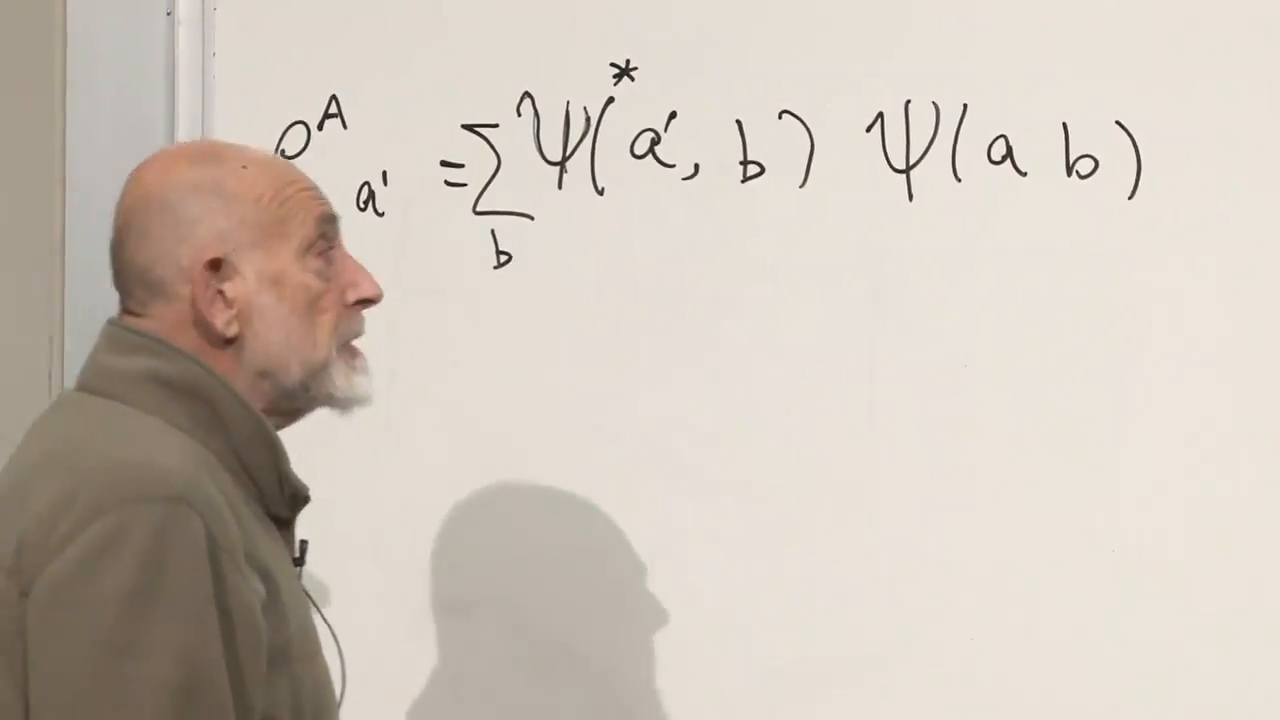
\includegraphics[width=0.88\textwidth]{lecture_08_figure_01.png}
\caption{結合波動関数をボブの基底ラベルについて和をとって作ったアリスの縮約密度行列。}
\lectureframe{00:04:34}
\end{figure}

ここでアリスの近傍とボブの近傍は広く解釈すべきである。それぞれに装置、磁場、技術者、その他その観測者が相互作用できる任意の自由度が含まれうる。局所性の主張は、ボブが自分の系を変えられないということではない。彼は多くの方法で変えてよい。主張は、彼が遠くにいる限り、彼が局所的に行う何ものも式~\eqref{eq:l8-reduced-density}を変えないということである。

\section{ボブの局所ユニタリ操作}

まずアリスを無視し、ボブの操作だけを記述する。ボブが磁場を変えるか、あるいは他の方法で自分の局所ハミルトニアンを変えるなら、彼の波動関数の係数はユニタリ変換を受ける。
\begin{equation}
\psi_M(b)
=
\sum_{b'}U_{bb'}\psi(b').
\label{eq:l8-bob-unitary}
\end{equation}
複合系の言葉では、アリスの添字は傍観者である。
\begin{equation}
\Psi_M(a,b)
=
\sum_{b'}U_{bb'}\Psi(a,b').
\label{eq:l8-composite-unitary}
\end{equation}
複素共役は、ケットの変換を対応するブラの変換に変える。
\begin{equation}
\Psi_M^*(a',b)
=
\sum_{b''}\Psi^*(a',b'')U^\dagger_{b''b}.
\label{eq:l8-composite-bra}
\end{equation}

\begin{figure}[htbp]
\centering
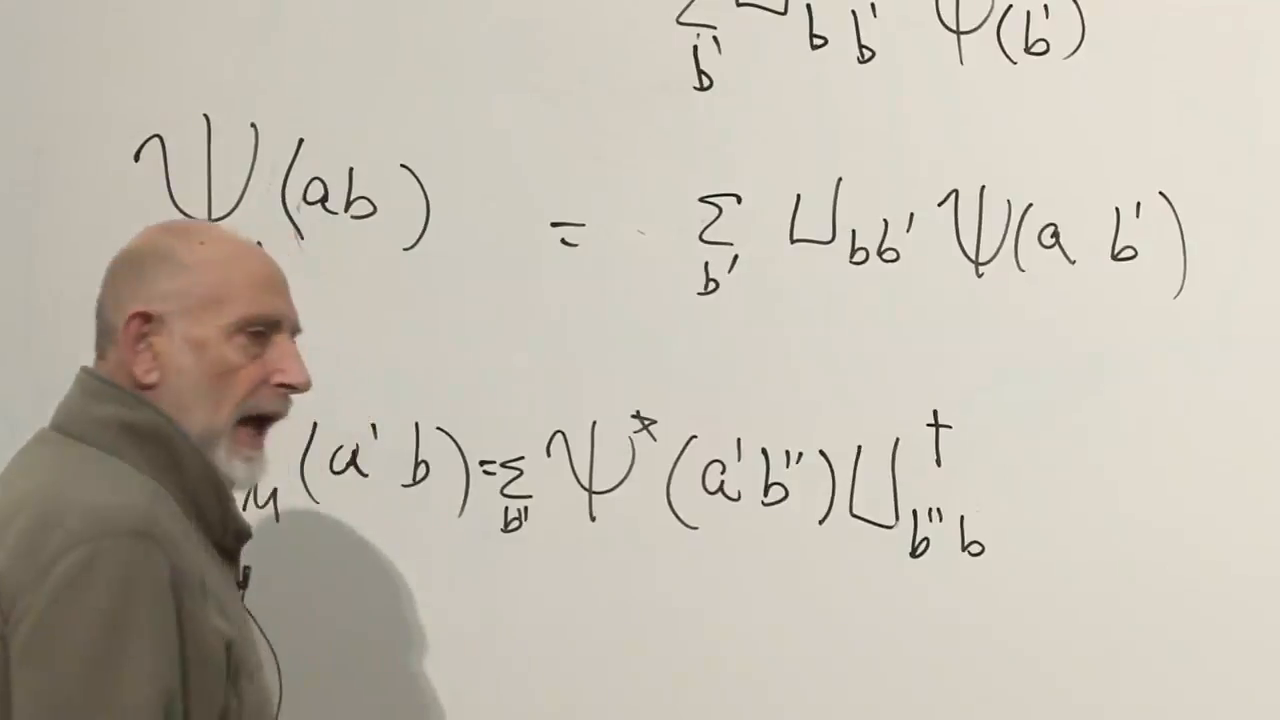
\includegraphics[width=0.88\textwidth]{lecture_08_figure_02.png}
\caption{ユニタリ行列はボブのケット添字に作用し、エルミート共役行列は対応するブラ添字に作用する。}
\lectureframe{00:12:54}
\end{figure}

ここでアリスの密度行列を再計算する。
\begin{align}
\rho_{A,M}(a',a)
&=
\sum_b\Psi_M^*(a',b)\Psi_M(a,b) \notag\\
&=
\sum_{b,b',b''}
\Psi^*(a',b'')
U^\dagger_{b''b}U_{bb'}
\Psi(a,b') \notag\\
&=
\sum_{b',b''}
\Psi^*(a',b'')
(U^\dagger U)_{b''b'}
\Psi(a,b') \notag\\
&=
\sum_{b',b''}
\Psi^*(a',b'')\delta_{b''b'}\Psi(a,b') \notag\\
&=
\sum_{b'}\Psi^*(a',b')\Psi(a,b') \notag\\
&=
\rho_A(a',a).
\label{eq:l8-locality-proof}
\end{align}

\begin{figure}[htbp]
\centering
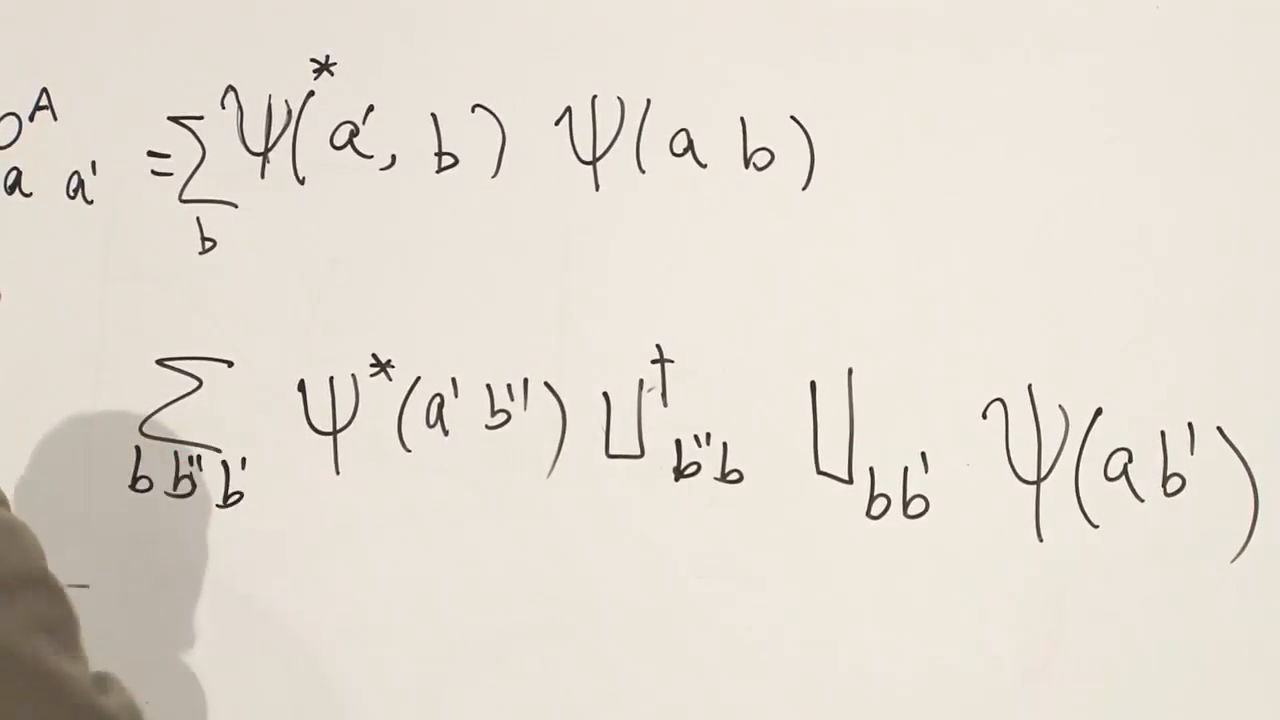
\includegraphics[width=0.88\textwidth]{lecture_08_figure_03.png}
\caption{黒板での局所性の計算：\(U^\dagger U\)はアリスの縮約状態の内部で恒等行列に収縮する。}
\lectureframe{00:14:27}
\end{figure}

証明全体はこの収縮である。
\begin{equation}
\sum_bU^\dagger_{b''b}U_{bb'}
=(U^\dagger U)_{b''b'}
=\delta_{b''b'}.
\label{eq:l8-unitarity-contraction}
\end{equation}
因数分解の仮定は一切用いていない。式~\eqref{eq:l8-locality-proof}は、結合状態が積状態であっても最大もつれ状態であっても成り立つ。したがって、アリスのみに関するすべての期待値、
\begin{equation}
\expect{L_A}
=
\operatorname{Tr}_A(\rho_A L_A),
\end{equation}
はボブの局所ユニタリ変換の下で不変である。

\begin{classroomqa}
\audiencequestion{ボブが自分のスピンに何かを行っているなら、なぜそれはすでにユニタリ性の破れではないのか？}
\lecturerresponse{何かを行うことは、非ユニタリ写像を適用することを意味しない。ボブは磁石を回転させ、局所ハミルトニアンを変え、あるいは自分のスピンを歳差運動させることができる。それらは通常のユニタリ発展である。それらは彼自身の状態と彼自身の結果確率を変えるが、上記の計算が示すように、アリスの縮約状態を変えることはない。}
\end{classroomqa}

\begin{classroomqa}
\audiencequestion{それでは量子力学は局所性に従うのか？}
\lecturerresponse{ここで用いた操作的な局所性には従う。すなわち、ボブは自分の近傍だけで作用して、アリスが利用できる測定の統計に影響を及ぼすことはできない。もつれた結合相関は非古典的であり続けるが、それらは制御可能な信号を与えない。}
\end{classroomqa}

\subsection{ユニタリ性が重要である理由}

ユニタリ性は装飾ではなかった。それは式~\eqref{eq:l8-unitarity-contraction}における恒等性を与えた。以前の言葉で言えば、ユニタリ性は区別の保存を表す。すなわち、二つの識別可能な状態ベクトルは可逆的発展の下でも識別可能なままである。もしボブがわずかでも非ユニタリな決定論的発展を持つなら、\(U^\dagger U\)は恒等行列にはならない。そのときアリスの縮約密度行列は直ちに変化し得て、ボブに光より速く信号を送る手段を与えることになる。

この密接な結びつきは、量子力学を部分的に修正することが難しい一つの理由である。発展則を変えれば、一見無関係な原理もそれとともに破れ得る。局所性、確率保存、可逆的な状態発展は一つの構造の部分である。

\begin{classroomqa}
\audiencequestion{非ユニタリ操作はどのようにして光より速い信号を可能にするのか？}
\lecturerresponse{ボブはそれを適用するか否かを選ぶであろう。もしその写像が\(\rho_A\)を変えるなら、アリスはアンサンブルに対する局所測定を繰り返すことで二つの選択を区別できる。その変化はボブから信号が伝播することなく生じるが、まさにそれをユニタリの相殺が防いでいる。}
\end{classroomqa}

\section{収縮は条件を変えるが、遠方の周辺分布は変えない}

ビームスプリッターの例はこの不安を生々しく示す。単一光子が二つの経路の重ね合わせに置かれ、一方はアリスへ、他方はボブへ向かう。アリスの検出器がクリックすれば、条件付き状態はボブの経路での後のクリックにゼロ振幅を割り当てる。アリスがボブの光子を瞬時に変えたと言いたくなる。

アリスの記録なしにボブが観測できるものは異なる。いかなるメッセージを受け取る前にも、彼はアリスの可能な結果について平均しなければならない。その無条件平均は彼の縮約密度行列によって記述され、それは変化しない。アリスのクリックは、彼女の結果が知られた後の一回のランを記述する条件付き部分アンサンブルを変えるが、ボブの局所周辺分布を変えることはない。
\begin{equation}
\rho_B
\qquad\text{and}\qquad
\rho_{B\mid A=\text{click}}
\end{equation}
の区別は、無信号性と有用な相関との区別である。

\begin{classroomqa}
\audiencequestion{一方の検出器がクリックすると、他方の腕の波動関数は瞬時にゼロに収縮しないのか？}
\lecturerresponse{そのクリックに条件付けられた状態は変化するが、遠方の観測者は通常のメッセージが届くまでその条件を有しない。ボブの無条件密度行列と彼のすべての平均局所統計は変わらない。収縮を電信に用いることはできない。}
\end{classroomqa}

\begin{classroomqa}
\audiencequestion{この混乱は、状態と状態に関する情報との混同の一部なのでしょうか。}
\lecturerresponse{その言い方は示唆的ではあるが、まだ緩すぎる。具体的な区別は、結合状態、縮約状態、そして報告された結果に条件づけられた状態の間の区別である。これら三つの数学的対象を別々に保つほうが、情報という語だけで問題を決着させようとするより安全である。}
\end{classroomqa}

それでもアインシュタイン--ポドルスキー--ローゼンの不快感は残る。一重項は、\emph{全体}について最大限の知識を与えうる一方で、どちらの構成要素も純粋な局所状態をもたない。この古典的期待の逆転---部分に確定した純粋状態を割り当てることなく全体を知る---は、シグナリング効果ではないが、真に特異である。その特異性をより鋭くあらわにするために、量子力学をプログラミング問題に変えてみよう。

\section{一つのスピンのための古典的シミュレータ}

コンピュータ画面上にスピン装置を描く。ユーザーはそれを向きづけ、測定ボタン\(M\)を押し、\(+1\)または\(-1\)を読み取ることができる。古典的コンピュータの内部には二つの複素振幅を格納する。
\begin{equation}
\alpha_u,\qquad \alpha_d,
\qquad
|\alpha_u|^2+|\alpha_d|^2=1.
\label{eq:l8-one-spin-amplitudes}
\end{equation}
測定と測定の間、コンピュータは適切なSchr\"odinger方程式を積分する。シミュレートされた磁場は、実際のスピン状態がそうするのとちょうど同じように振幅を歳差運動させることができる。

\begin{figure}[htbp]
\centering
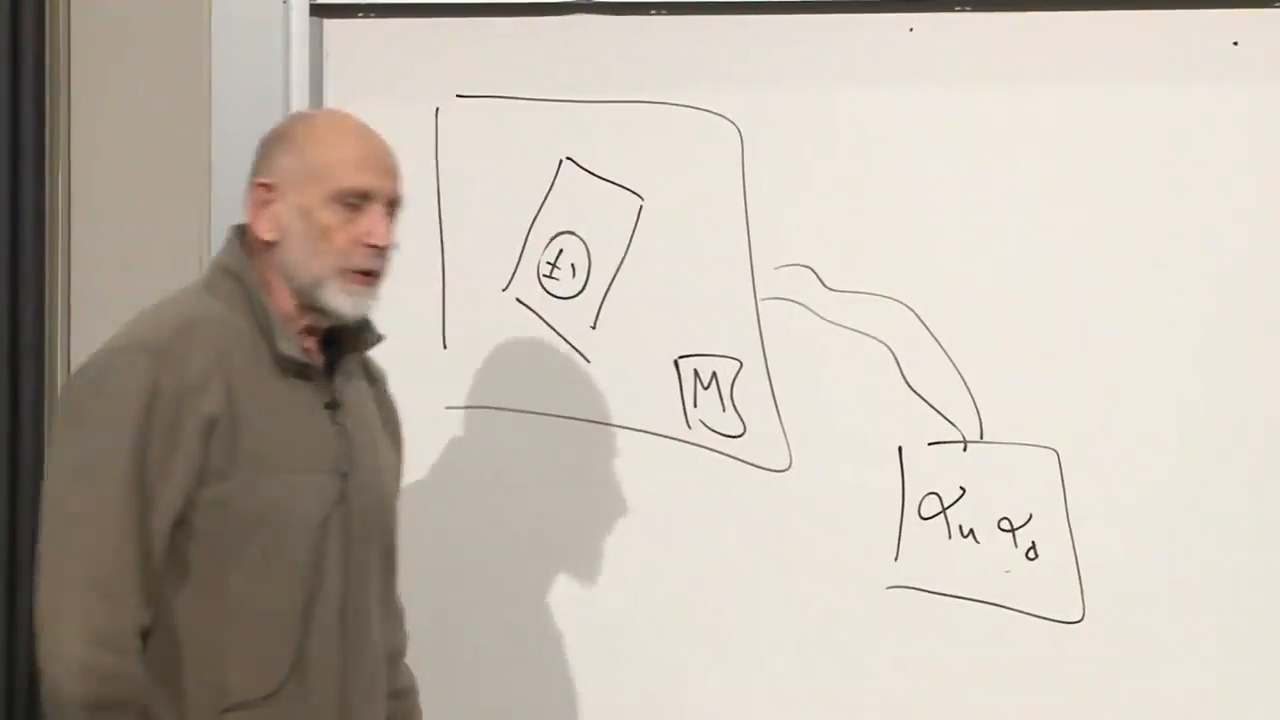
\includegraphics[width=0.88\textwidth]{lecture_08_figure_04.png}
\caption{一スピンシミュレータ：向きづけ可能な装置と測定ボタンが、二つの振幅を格納するコンピュータに接続されている。}
\lectureframe{00:27:47}
\end{figure}

ユーザーが\(M\)を押すと、擬似乱数生成器がボルンの確率
\begin{equation}
P(+1)=|\alpha_u|^2,
\qquad
P(-1)=|\alpha_d|^2.
\label{eq:l8-one-spin-born}
\end{equation}
で結果を選ぶ。コンピュータは選ばれた符号を表示し、その後、状態更新を行う。\(+1\)の後では、
\begin{equation}
(\alpha_u,\alpha_d)\longrightarrow(1,0),
\end{equation}
であるのに対し、\(-1\)の後では、
\begin{equation}
(\alpha_u,\alpha_d)\longrightarrow(0,1).
\end{equation}
である。その後、測定後の状態からユニタリ発展を再開する。ユーザーが\(M\)を押す前に装置を回転させれば、コンピュータは基底を変え、新しい軸に適した確率を計算する。

ハードウェアに特に量子的なものは要求されない。決定論的な擬似乱数アルゴリズムで、ユーザーにはランダムに見える系列を生成するのに十分である。一つのスピンについては、この古典的模倣は実験室の実験と操作上区別できないものになりうる。

\begin{classroomqa}
\audiencequestion{測定ボタンの目的は何か。それを押す前に経過した時間は重要か。}
\lecturerresponse{ボタンは、シミュレータがボルン分布をサンプリングし、格納された振幅を更新する瞬間を印づける。待っている間、振幅はハミルトニアンのもとで発展する。ハミルトニアンがゼロなら時間とともに何も変化しないが、磁場があればシミュレートされたスピンは測定前に歳差運動する。}
\end{classroomqa}

\begin{classroomqa}
\audiencequestion{いつボタンを押すか、あるいは装置をどちらに向けるかを決めるのは誰か。}
\lecturerresponse{このモデルでは、実験者がそれらの設定を与える。シミュレータは状態を連続的に追跡し、ボタンが押されたときに選択された軸と測定時刻を用いる。設定が準備された対から独立に選べるという仮定には、後の議論で再び戻る。}
\end{classroomqa}

\section{二つのスピン：局所シミュレーションが失敗する場所}

積状態にある二つのスピンは依然として容易である。アリスに振幅\(\alpha_u,\alpha_d\)を格納するコンピュータを一つ与え、ボブに\(\beta_u,\beta_d\)を格納する別のコンピュータを与える。各機械は自分のスピンを発展させ測定する。結合係数が因数分解するので、通信は必要ない。
\begin{equation}
\Psi(a,b)=\alpha_a\beta_b.
\end{equation}

任意の二スピン状態には四つの係数が必要である。
\begin{equation}
\alpha_{uu},\qquad
\alpha_{ud},\qquad
\alpha_{du},\qquad
\alpha_{dd},
\qquad
\sum_{a,b}|\alpha_{ab}|^2=1.
\label{eq:l8-four-amplitudes}
\end{equation}
単一の中央コンピュータがこれらの数を格納し、四次元のSchr\"odinger方程式でそれらを発展させることができる。どちらかの観測者が測定すると、中央機械は正しい周辺確率をサンプリングし、両立しない成分を捨て、生き残った成分を再規格化し、条件付き状態から続行する。

\begin{figure}[htbp]
\centering
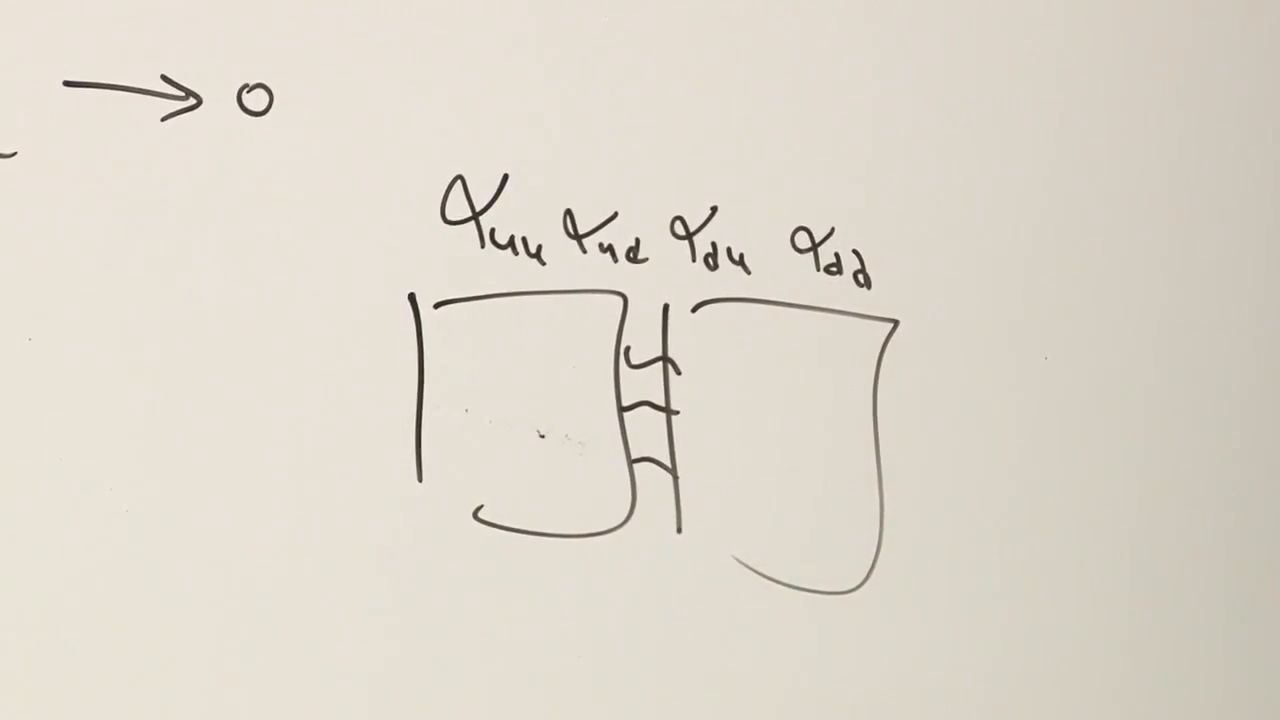
\includegraphics[width=0.88\textwidth]{lecture_08_figure_05.png}
\caption{中央シミュレータは任意の二スピン状態の四つの振幅を格納し、両方の測定ステーションに接続されたままである。}
\lectureframe{00:37:47}
\end{figure}

この構成は、中央プロセッサが両側に接続されたままである限り、もつれを完全にシミュレートする。問題は、四つの振幅を二つの機械にコピーし、それらを分離し、配線を切り、各機械に独自の乱数生成器を使わせたときに始まる。一重項については、
\begin{equation}
\ket{\Psi^-}
=
\frac{1}{\sqrt2}
\left(
\ket{u}_A\ket{d}_B-\ket{d}_A\ket{u}_B
\right),
\label{eq:l8-singlet}
\end{equation}
等しい軸での測定は反対でなければならない。独立なランダム選択は代わりに\(++\)または\(--\)を生じうるので、両方の機械が結合係数のコピーから始めたにもかかわらず、相関は失われる。

\begin{classroomqa}
\audiencequestion{二つの装置は分離される前に一つの乱数源を共有できるだろうか。}
\lecturerresponse{共有された乱数性は、一つの固定された測定軸に対する所定の相関を実現しうる。より深いベル問題は、独立に選ばれたあらゆる軸の対に対して量子相関を再現する一つの局所的な枠組みを問うている。あらかじめ読み込まれた共有変数はベル局所模型に含まれ、そのような模型は完全な量子相関関数を再現しない。}
\end{classroomqa}

\begin{classroomqa}
\audiencequestion{四つの振幅は独立だろうか。}
\lecturerresponse{それらは一つの規格化された結合状態の四つの座標であり、四つの独立な局所状態ではない。もつれた状態ではそれらを\(\alpha_a\beta_b\)と書くことはできない。局所的な結果が選ばれた後、生き残った結合係数はコヒーレントに更新されなければならない。二つの切り離されたコピーは自動的に整合する更新を行うわけではない。}
\end{classroomqa}

\subsection{隠れた配線が意味するもの}

両方の局に接続された中央の乱数発生器は出力を調整しうる。通常の古典的シミュレータでは、それらの配線は通信路でもある。ボブは故意にアリスへビットを送ることができ、そのリンクが瞬時であれば、その装置は局所性を破ることになる。

量子系はボブにその自由を与えない。彼に許された局所変換はユニタリであり、縮約密度行列による証明はすでに、そのような変換がアリスの周辺統計を変えないことを示していた。したがってシミュレータの配線は、通常の古典的記帳が誤った構造をもつことの徴候であり、自然が利用可能な超光速ケーブルを含む証拠ではない。

\begin{classroomqa}
\audiencequestion{古典的シミュレータに必要な配線は物理的な非局所性を表すのか。}
\lecturerresponse{それらは素朴な古典模型が必要とする余分な調整を表している。それらが通常の使用可能な配線であれば、シグナリングを許すことになり、量子実験を模型化しない。より安全な結論は、局所古典シミュレーションと量子力学は異なる論理構造をもつということであり、隠れた通信配線が発見されたということではない。}
\end{classroomqa}

\begin{classroomqa}
\audiencequestion{アリスとボブがそれぞれランダムなビットを受け取るが、そのビットが完全に相関しているとしたら、そのどこが奇妙なのか。}
\lecturerresponse{一つのあらかじめ取り決められた相関については何も奇妙ではない。同一の封筒や共有された乱数種がそれを生みうる。非古典的な内容は、アリスとボブが両立しない設定の中から独立に選び、その結果得られる相関がベル不等式を破り、しかも各局所結果がランダムのままであるときに現れる。}
\end{classroomqa}

この思考実験には、明るみに出す価値のある前提も含まれている。測定設定は独立な選択として扱われる。アリスとボブは、いつボタンを押すか、装置をどのように向けるかを決めるが、それらの選択は源の変数によって密かに固定されてはいない。観測者とその決定機構を一つの閉じた物理系の内部に含めると、自由選択という哲学的言辞は微妙になる。操作的なベルテストは、必要な条件を測定独立性として定式化し、空間的に隔たった、外部で生成された設定を用意する。講義は形而上学を開いたままにしつつ、実験的前提を保持する。

\begin{classroomqa}
\audiencequestion{アリスとボブを物理系の内部に置くことは抜け穴を生むのか。}
\lecturerresponse{それは一つの仮定を露わにする。設定は、対を準備する隠れた変数とあらかじめ相関していてはならない。自由意志を論じることはできるが、検証可能な言明は測定独立性である。それを放棄することは論理的に可能だが、通常の局所シミュレーションを与えるのではなく、説明の負担を変えるだけである。}
\end{classroomqa}

\section{スピンから直線上の粒子へ}

スピンは、有限次元ベクトルからもつれと局所性に至るまで議論を導いてきた。ここでヒルベルト空間を拡大する。無限に長い直線上を運動する一つの粒子を考える。位置固有状態は
\begin{equation}
\ket{x},
\end{equation}
と表され、粒子が確定した位置\(x\)をもつことを意味する。これらのケットは連続的にラベル付けされた基底をなす。一般の状態はそれらの重ね合わせであり、その位置空間波動関数は
\begin{equation}
\psi(x)=\braket{x}{\Psi}.
\label{eq:l8-position-wavefunction}
\end{equation}

\begin{figure}[htbp]
\centering
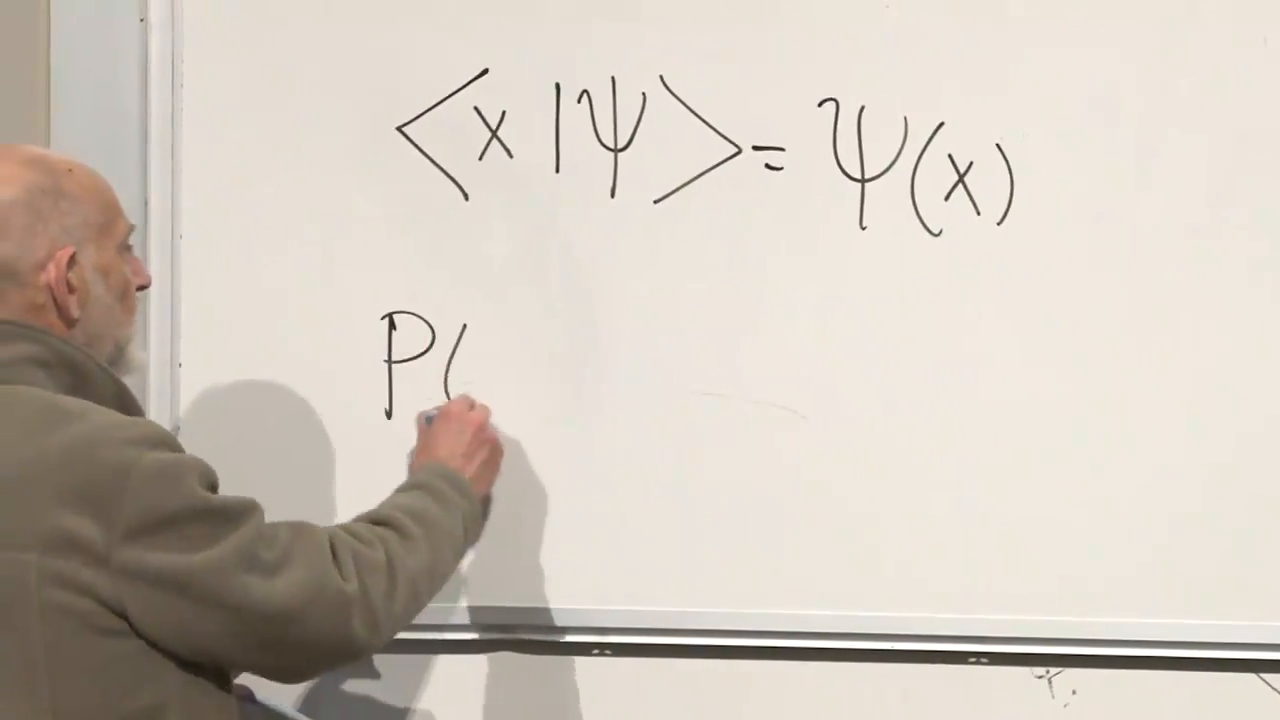
\includegraphics[width=0.88\textwidth]{lecture_08_figure_06.png}
\caption{位置空間波動関数は、抽象的な状態を基底ケット\(\ket{x}\)へ射影したものである。}
\lectureframe{00:56:51}
\end{figure}

位置は完全な基底ラベルとして用いられている。これは、古典的状態が位置だけで指定できるということでも、粒子が確定した位置と運動量を同時にもつということでもない。すべての量子状態ベクトルは位置基底で展開できるということである。運動量は、それらの位置空間係数に作用する演算子として現れる。

ボルンの規則により、確率\emph{密度}が得られる。
\begin{equation}
\rho(x)=|\psi(x)|^2.
\label{eq:l8-probability-density}
\end{equation}
連続変数に対しては、厳密に一点における確率は通常ゼロである。粒子がある区間内に見出される確率は
\begin{equation}
P(x_1<x<x_2)
=
\int_{x_1}^{x_2}|\psi(x)|^2\,dx,
\end{equation}
であり、規格化には
\begin{equation}
\int_{-\infty}^{\infty}|\psi(x)|^2\,dx=1.
\label{eq:l8-continuous-normalization}
\end{equation}
が必要である。

\begin{classroomqa}
\audiencequestion{古典的な粒子が位置と運動量の両方を必要とするのに、なぜ位置だけで完全な基底となり得るのか。}
\lecturerresponse{ここでの完全性は量子ベクトルの表現に関するものである。すべての\(x\)に対する係数\(\psi(x)\)が状態を指定し、運動量の情報はそれらの位相と空間的変化に符号化されている。位置と運動量は異なる基底であり、後にフーリエ変換によって関係づけられる。それらは同時的な古典的ラベルではない。}
\end{classroomqa}

\begin{classroomqa}
\audiencequestion{\(|\psi(x)|^2\)は粒子が厳密に点\(x\)に見出される確率か。}
\lecturerresponse{それは密度である。小さな区間\(dx\)を掛けるとその区間における近似確率が得られ、積分すると有限領域に対する厳密な確率が得られる。密度は、一つの孤立点に割り当てられる確率がゼロであっても、非ゼロであり得る。}
\end{classroomqa}

\section{連続的な正規直交性とデルタ関数}

離散的な正規直交基底に対しては、
\begin{equation}
\braket{a}{a'}=\delta_{aa'}.
\end{equation}
連続基底に対する類似は
\begin{equation}
\braket{x}{x'}=\delta(x-x'),
\label{eq:l8-delta-normalization}
\end{equation}
であり、ここでディラックのデルタは\(x\neq x'\)に対して消え、単位面積を持つ。
\begin{equation}
\int_{-\infty}^{\infty}\delta(x-x')\,dx'=1.
\end{equation}
幅\(\epsilon\)、高さ\(1/\epsilon\)、面積固定の狭いスパイクとして描き、\(\epsilon\to0\)の極限をとると考えてもよい。

\begin{figure}[htbp]
\centering
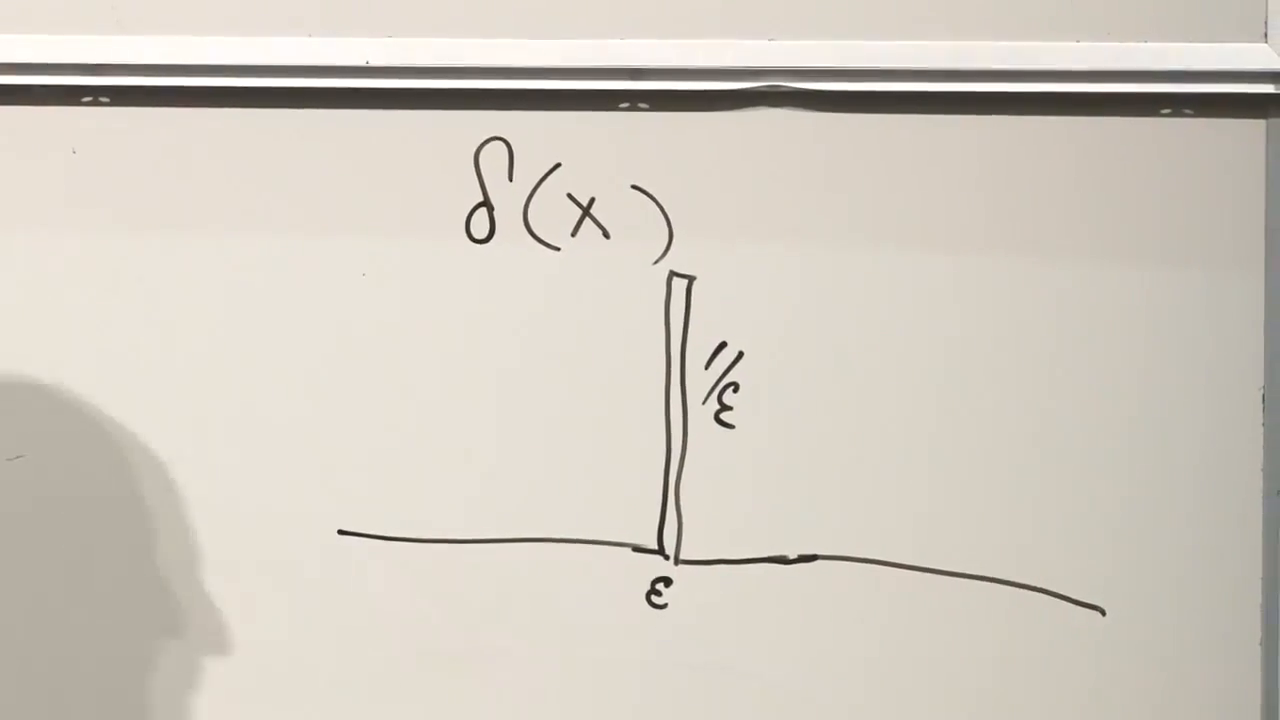
\includegraphics[width=0.88\textwidth]{lecture_08_figure_07.png}
\caption{ディラックのデルタの黒板における狭いスパイク表現：幅\(\epsilon\)、高さ\(1/\epsilon\)、単位面積。}
\lectureframe{01:01:57}
\end{figure}

この記法は超関数的な略記である。位置固有ケットは通常の二乗可積分ヒルベルト空間における規格化可能なベクトルではなく、積分の下でデルタ規格化が意味を持つ一般化ベクトルである。中心となる作業規則は
\begin{equation}
\int_{-\infty}^{\infty}
\delta(x-x')f(x')\,dx'
=f(x).
\label{eq:l8-delta-sampling}
\end{equation}
である。デルタはその引数が消える値の選択を行う。

次に連続的な展開を書く。
\begin{equation}
\ket{\Psi}
=
\int_{-\infty}^{\infty}
\psi(x')\ket{x'}\,dx'.
\label{eq:l8-continuous-expansion}
\end{equation}
\(\bra{x}\)を作用させると
\begin{align}
\braket{x}{\Psi}
&=
\int dx'\,\psi(x')\braket{x}{x'} \notag\\
&=
\int dx'\,\psi(x')\delta(x-x') \notag\\
&=
\psi(x).
\label{eq:l8-expansion-consistency}
\end{align}
が得られる。したがって、展開における係数と射影\(\braket{x}{\Psi}\)は、離散基底の場合と全く同様に、同じ関数である。

\begin{figure}[htbp]
\centering
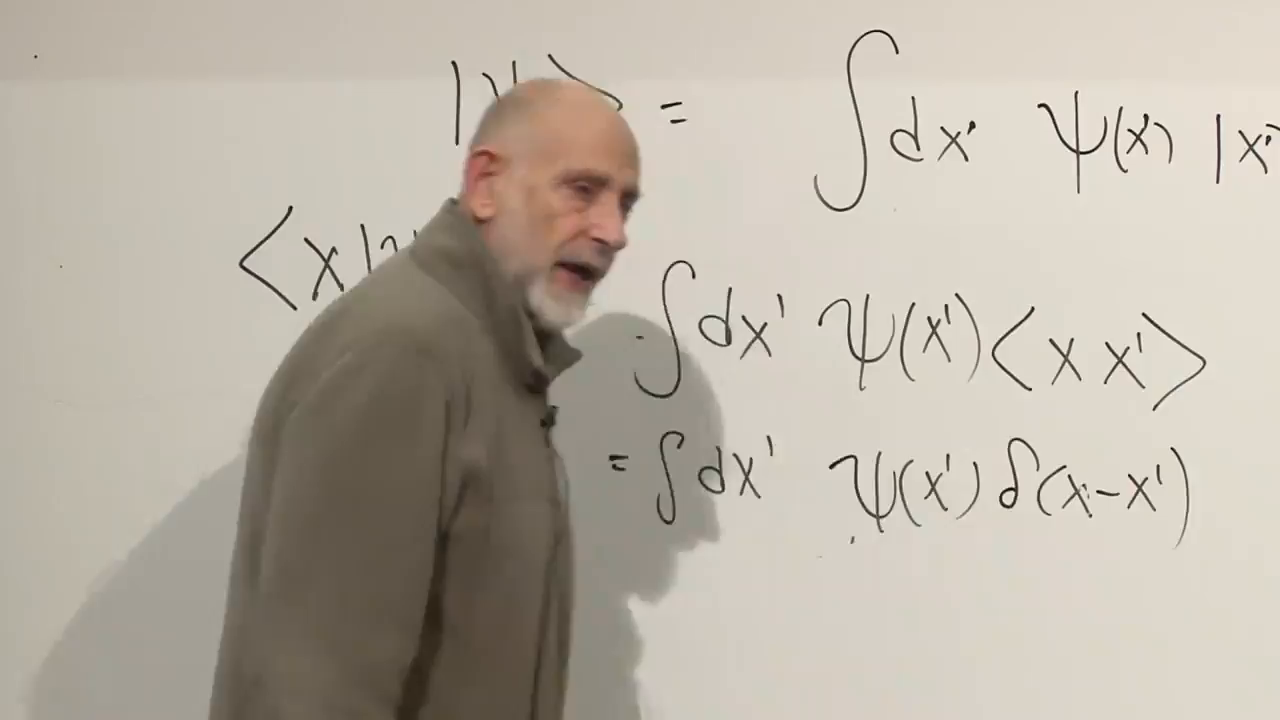
\includegraphics[width=0.88\textwidth]{lecture_08_figure_08.png}
\caption{連続的な状態展開と、\(\braket{x}{x'}=\delta(x-x')\)を用いたその整合性の確認。}
\lectureframe{01:07:00}
\end{figure}

\begin{classroomqa}
\audiencequestion{\(\psi(x')\)は有限次元ベクトルにおける振幅と同じ役割を果たすのか。}
\lecturerresponse{はい。基底ラベル\(a'\)は連続ラベル\(x'\)になり、和は積分になり、係数\(\psi(a')\)は関数\(\psi(x')\)になる。根底にあるベクトル空間としての主張は変わらない。}
\end{classroomqa}

\begin{classroomqa}
\audiencequestion{ディラックのデルタは本当に一点で無限の値を持つ関数なのか。}
\lecturerresponse{その描像は有用だが、文字通りのものではない。厳密には、デルタは積分の下での作用によって定義される超関数であり、式~\eqref{eq:l8-delta-sampling}で与えられる。狭い単位面積のスパイクは、同じサンプリング規則に近づく通常の関数の列である。}
\end{classroomqa}

\section{関数をベクトルとして}

内積を見るために、まず離散的な計算を思い出そう。
\begin{align}
\braket{\psi}{\phi}
&=
\sum_{a',a}
\psi^*(a')\braket{a'}{a}\phi(a) \notag\\
&=
\sum_a\psi^*(a)\phi(a).
\label{eq:l8-discrete-inner-product}
\end{align}
複素共役をとった係数はブラに属し、正規直交性が二重和を潰す。

\begin{figure}[htbp]
\centering
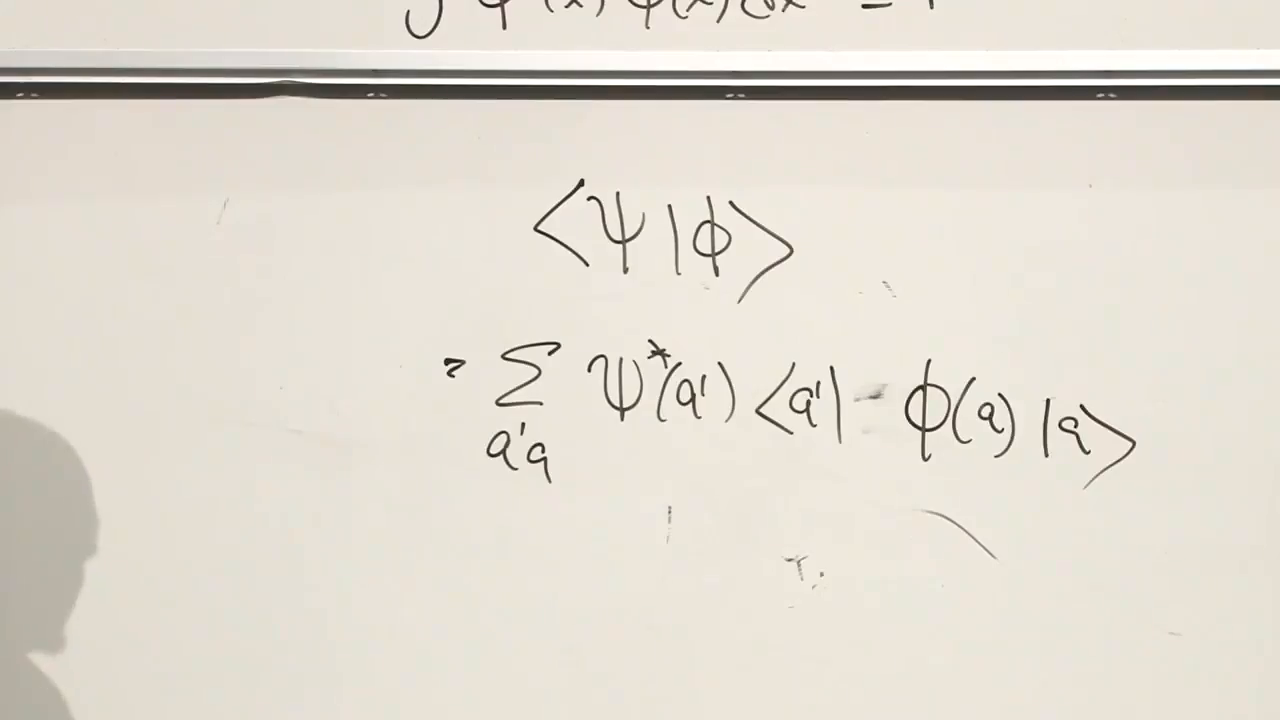
\includegraphics[width=0.88\textwidth]{lecture_08_figure_09.png}
\caption{和が積分に置き換えられる前に、基底で展開された離散的内積。}
\lectureframe{01:11:11}
\end{figure}

基底ラベルを位置に、和を積分に置き換える。
\begin{equation}
\braket{\psi}{\phi}
=
\int_{-\infty}^{\infty}\psi^*(x)\phi(x)\,dx.
\label{eq:l8-continuous-inner-product}
\end{equation}
ベクトルの順序を入れ替えると答えは複素共役になり、
\begin{equation}
\braket{\phi}{\psi}
=
\braket{\psi}{\phi}^*,
\end{equation}
ノルムは
\begin{equation}
\|\psi\|^2=\braket{\psi}{\psi}
=\int |\psi(x)|^2\,dx.
\end{equation}
である。

したがって関数はベクトルである。それらは加算され、複素スカラー倍され、規格化され、内積によって対にされることができる。無限直線上の物理的波動関数は二乗可積分であるから、無限遠で非有界に増大する関数は排除される。一般化基底関数\(\delta(x-x_0)\)はそのヒルベルト空間のちょうど外側に位置するが、超関数的基底ベクトルとして不可欠なままである。

\begin{classroomqa}
\audiencequestion{無印の積分限界は\(-\infty\)と\(+\infty\)であるべきか。}
\lecturerresponse{はい、無限直線に対してはそうである。これらの限界は、規格化可能な波動関数が十分速く減衰しなければならない理由も説明する。そうでなければ全確率積分が存在しないからである。}
\end{classroomqa}

\begin{classroomqa}
\audiencequestion{黒板に書いた式の一つに縦棒が欠けていた。それで意味は変わるのか。}
\lecturerresponse{単なる表記上のミスである。基底の重なりは\(\braket{a'}{a}\)であり、左にブラ、右にケットが置かれている。縦棒を復元すれば、その式が曖昧な行や列ではなく内積であることが明確になる。}
\end{classroomqa}

\begin{classroomqa}
\audiencequestion{ほとんどのものは大抵の時間、環境と絡み合っているのか。}
\lecturerresponse{現実的な巨視的条件では、その通りである。系は光子、空気分子、その他の自由度によって絶えず叩かれ、位相情報を環境へ広げていく。この環境との絡み合いがデコヒーレンスの中心であり、巨視的な選択肢の間の干渉が観測しにくい理由でもある。}
\end{classroomqa}

\begin{classroomqa}
\audiencequestion{超関数の数学的理論は物理学を変えたのか、それともデルタ関数をまともなものにしただけなのか。}
\lecturerresponse{その直接の役割は、物理学者がすでに用いていた操作を厳密にすることであった。超関数のための精密な言語を提供し、数学者との議論を減らしたが、それ自体で量子場の理論における超関数的困難のすべてを解決したわけではない。}
\end{classroomqa}

\section{波動関数上の線形演算子}

線形演算子は重ね合わせを保ちながら一つの関数を別の関数へ写す：
\begin{equation}
L(c_1\psi+c_2\phi)
=
c_1L\psi+c_2L\phi.
\end{equation}
観測量はエルミート演算子によって表されなければならない。現在の表記では、その条件は
\begin{equation}
\braket{\phi}{L\psi}
=
\braket{L\phi}{\psi},
\label{eq:l8-hermitian-condition}
\end{equation}
あるいは等価的に
\begin{equation}
\braket{\phi}{L\psi}
=
\braket{\psi}{L\phi}^*.
\end{equation}
である。非有界演算子の場合、この主張には定義域と境界条件が含まれる。以下の積分では、境界項が消える波動関数を仮定している。

\subsection{掛け算による位置}

最も単純な演算子は波動関数に座標を掛ける：
\begin{equation}
(x\psi)(x)=x\psi(x).
\label{eq:l8-position-operator}
\end{equation}
これは線形であり、
\begin{align}
\braket{\phi}{x\psi}
&=
\int dx\,\phi^*(x)x\psi(x), \notag\\
\braket{x\phi}{\psi}
&=
\int dx\,[x\phi(x)]^*\psi(x) \notag\\
&=
\int dx\,\phi^*(x)x\psi(x),
\end{align}
なぜなら\(x\)は実数だからである。したがって\(x\)を掛けることはエルミートであり、位置観測量を表す。

\begin{figure}[htbp]
\centering
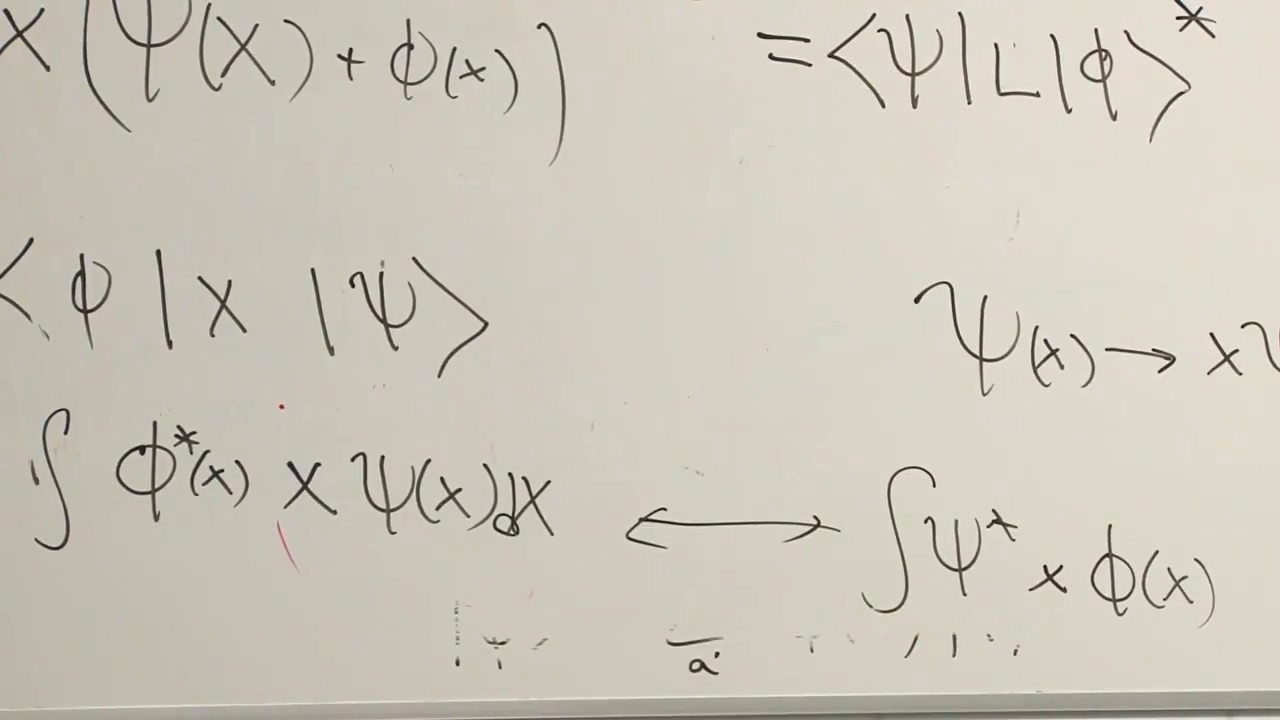
\includegraphics[width=0.88\textwidth]{lecture_08_figure_10.png}
\caption{位置演算子のエルミート性の検査。波動関数に実変数\(x\)を掛けるものと見なす。}
\lectureframe{01:26:47}
\end{figure}

\begin{classroomqa}
\audiencequestion{\(x\psi(x)\)において、\(x\)は演算子なのか、それとも単なる実数なのか。}
\lecturerresponse{各点では実数の座標値であるが、関数全体\(\psi(x)\)を新しい関数\(x\psi(x)\)へ写す規則が演算子である。その実数性こそが、エルミート性の検査における二つの内積を一致させる。}
\end{classroomqa}

\subsection{微分は反エルミートである}

微分を試してみる：
\begin{equation}
D=\frac{d}{dx}.
\end{equation}
これは線形であるが、部分積分により
\begin{align}
\braket{\phi}{D\psi}
&=
\int dx\,\phi^*(x)\frac{d\psi}{dx} \notag\\
&=
\left[\phi^*(x)\psi(x)\right]_{-\infty}^{\infty}
-
\int dx\,\frac{d\phi^*}{dx}\psi(x) \notag\\
&=
-\braket{D\phi}{\psi},
\label{eq:l8-derivative-adjoint}
\end{align}
が得られる。ここで境界項は消える。したがって
\begin{equation}
D^\dagger=-D.
\end{equation}
微分はエルミートではなく反エルミートである。

\begin{figure}[htbp]
\centering
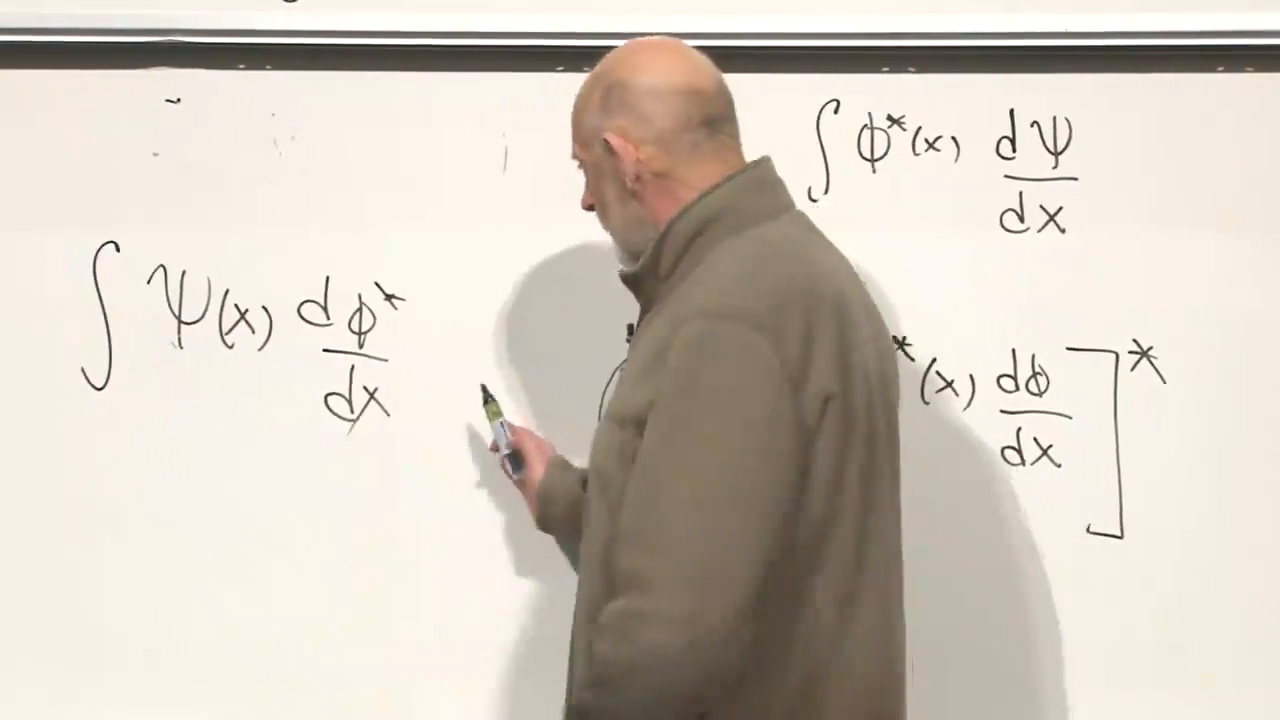
\includegraphics[width=0.88\textwidth]{lecture_08_figure_11.png}
\caption{部分積分は二つの波動関数の間で微分を移し、決定的な負符号を導入する。}
\lectureframe{01:32:30}
\end{figure}

\(-i\)を掛ける：
\begin{equation}
p=-i\frac{d}{dx}.
\label{eq:l8-momentum-natural-units}
\end{equation}
複素共役は\(-i\)を\(+i\)に変え、部分積分はもう一つの負符号をもたらす。符号が打ち消し合うので\(p^\dagger=p\)となる。単位を戻すと、
\begin{equation}
p=-i\hbar\frac{d}{dx}.
\label{eq:l8-momentum-operator}
\end{equation}

期待値はその実数性を明示する：
\begin{align}
\expect{p}_\psi
&=
-i\int dx\,\psi^*(x)\frac{d\psi}{dx} \notag\\
&=
i\int dx\,\frac{d\psi^*}{dx}\psi(x) \notag\\
&=
\expect{p}_\psi^*.
\label{eq:l8-momentum-expectation-real}
\end{align}
自身の複素共役に等しい数は実数であり、観測量の期待値はそうでなければならない。

\begin{figure}[htbp]
\centering
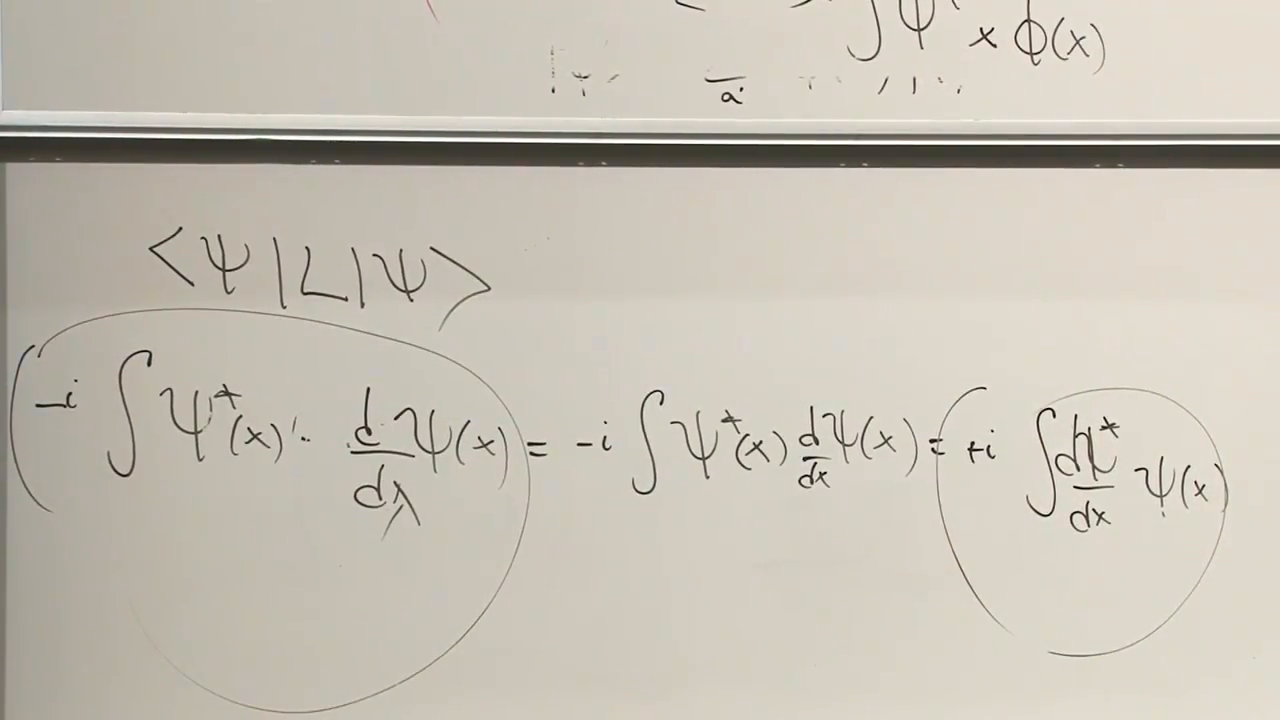
\includegraphics[width=0.88\textwidth]{lecture_08_figure_12.png}
\caption{部分積分の前後での運動量期待値。二つの形は複素共役であり、等しい。}
\lectureframe{01:39:44}
\end{figure}

\begin{classroomqa}
\audiencequestion{なぜ\(i\)を含む演算子が実の観測量を表せるのか。}
\lecturerresponse{エルミート性は内積の下での演算子全体に関わるものであり、その座標表示の式に現れるすべての記号が実数かどうかではない。因子\(i\)は、部分積分によって微分を移すときに得られる負符号を補償し、すべての期待値を実数にする。}
\end{classroomqa}

\section{正準交換子}

もう一つの計算が、式~\eqref{eq:l8-momentum-operator}の演算子がなぜ注目に値するかを明らかにする。\(\hbar=1\)とする単位で、まず\(x\)を作用させ、次に\(p\)を作用させる：
\begin{align}
(px\psi)(x)
&=
-i\frac{d}{dx}\bigl(x\psi(x)\bigr) \notag\\
&=
-i\psi(x)-ix\frac{d\psi}{dx}.
\label{eq:l8-px}
\end{align}
順序を逆にする：
\begin{equation}
(xp\psi)(x)
=
-ix\frac{d\psi}{dx}.
\label{eq:l8-xp}
\end{equation}
式~\eqref{eq:l8-px}から式~\eqref{eq:l8-xp}を引くと、
\begin{equation}
\bigl([x,p]\psi\bigr)(x)
=
\bigl(xp-px\bigr)\psi(x)
=
i\psi(x).
\end{equation}
これが演算子の定義域内のすべての波動関数について成り立つので、
\begin{equation}
[x,p]=i,
\end{equation}
あるいは単位を戻すと、
\begin{equation}
[x,p]=i\hbar.
\label{eq:l8-canonical-commutator}
\end{equation}

\begin{figure}[htbp]
\centering
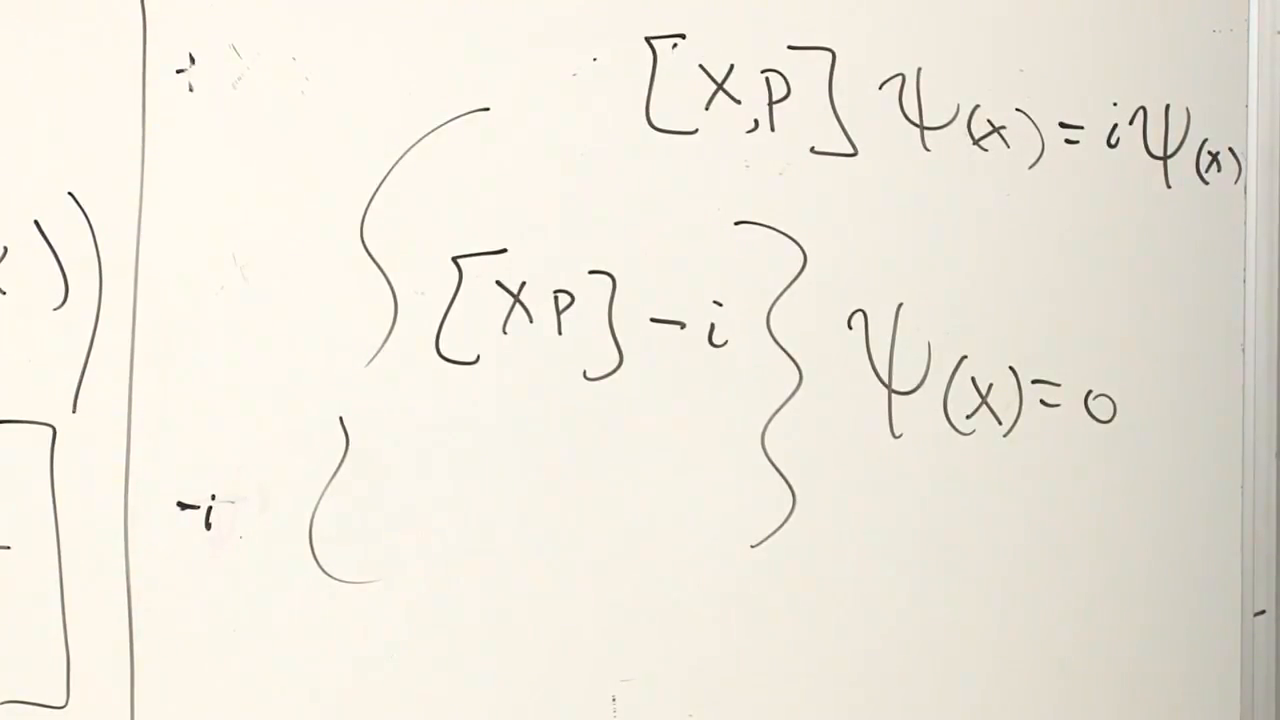
\includegraphics[width=0.88\textwidth]{lecture_08_figure_13.png}
\caption{完成した演算子の議論：すべての波動関数について\(([x,p]-i)\psi=0\)ならば、\([x,p]=i\)である。}
\lectureframe{01:46:24}
\end{figure}

古典的な対応物は
\begin{equation}
\{x,p\}_{\mathrm{PB}}=1.
\end{equation}
である。ディラックの歴史的な推論は、現在の導出とは逆の方向に進んだ。彼は反対称なポアソン括弧と交換子の代数的類似から出発し、対応
\begin{equation}
[A,B]\longleftrightarrow i\hbar\{A,B\}_{\mathrm{PB}},
\end{equation}
を仮定して、運動量演算子が位置との正準交換関係を満たさなければならないと推論した。ここでは、微分のエルミート性の破れを修復することによって\(-i\,d/dx\)を発見し、その後になって初めて同じ代数を見出したのである。

\begin{classroomqa}
\audiencequestion{交換関係だけで\(-i\hbar\,d/dx\)が物理的な運動量であることが証明されるのか。}
\lecturerresponse{それは強い証拠ではあるが、物理的な同定のすべてではない。依然として、この演算子が空間並進を生成すること、並進対称性が存在するときにその期待値が保存されること、そして適切な非相対論的系において波束が群速度\(\expect{p}/m\)で運動することを示さなければならない。}
\end{classroomqa}

\section{次に来るもの}

スピンから粒子への移行は、その構造を保ちながらスケールを変えてきた。連続的にラベル付けされた基底が、有限個の基底ベクトルのリストを置き換える。和は積分になり、クロネッカーのデルタはディラックのデルタになり、列ベクトルは二乗可積分関数になる。位置は掛け算として作用し、運動量は微分として作用する。

次の課題は単なる記法上のものではなく物理的なものである。運動量の確率には運動量基底とフーリエ変換が必要である。時間発展には\(\psi(x,t)\)に対するSchr\"odinger方程式が必要である。そうすれば波束が抽象的な演算子\(p=-i\hbar\,d/dx\)を運動に結びつける。すなわち、その群速度は運動量を質量で割ったものと関係づけられ、並進対称性が運動量保存を説明する。したがって交換関係\([x,p]=i\hbar\)は孤立した技巧ではない。それはすでに展開されたベクトル空間の力学と、粒子の量子力学をつなぐ蝶番なのである。
